%------------------------------------------------------------------------------
% Author(s):
% Varaun Ramgoolie
%
% Copyright:
%  Copyright (C) 2020 Brad Bachu, Arjun Mohammed, Varaun Ramgoolie, Nicholas Sammy
%
%  This file is part of Applied-Mathematics-Unit2 and is distributed under the
%  terms of the MIT License. See the LICENSE file for details.
%
%  Description:
%     Year: 2014 drawing of graph for q5 (a)(i)
%     Module: 3
%     Question: 5
%------------------------------------------------------------------------------
\documentclass[crop,tikz]{standalone}
\usepackage{pgfplots}
\usepackage{../../../../src/tikzappmath}
\usetikzlibrary{patterns}

\begin{document}
	
	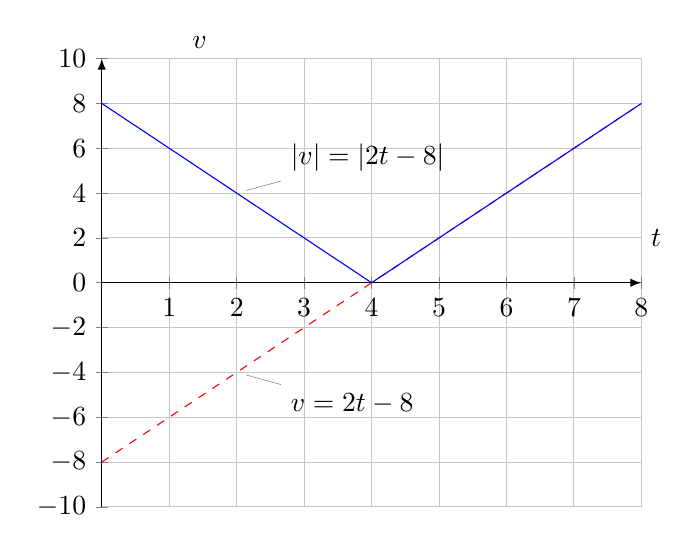
\begin{tikzpicture}[scale=1]
		
		\begin{axis}
			[
			xmin=0,xmax=8,
			ymin=-10,ymax=10,
			grid=both,
			grid style={line width=0pt, draw=darkgray!10},
			major grid style={line width=0pt,draw=darkgray!30},
			axis lines=left,
			minor tick num=0,
			enlargelimits={abs=0},
			axis line style={-latex},
			axis x line shift=-10,
			samples=1,
			domain = -2:2,
			ytick={-10,-8,...,10},
			xtick={1,...,8},
			xlabel={$t$},
			ylabel={$v$},
			x label style={at={(axis description cs:1,0.64)},anchor=north west},
			y label style={at={(axis description cs:0.15,1)},anchor=south west, rotate=-90}
			]
			
			
			\addplot [domain=0:8, samples=100, color=red, dashed]{2*x-8};

			\addplot [domain=0:4, samples=100, color=blue,]{8-2*x};		
			
			\addplot [domain=4:8, samples=100, color=blue,]{2*x-8};

			\node [pin=15:{$|v|=|2t-8|$}] at (axis cs:(2,4) {};
			
			\node [pin=-15:{$v=2t-8$}] at (axis cs:(2,-4) {};
			
		\end{axis}	
		
	\end{tikzpicture}
	
\end{document}